\chapter{Estereoquímica aprofundada}\label{ch:b1:stereochemistry-in-depth}

Esmague algumas sementes de alcaravia e, depois, uma folha de hortelã:
dois cheiros bem diferentes. O principal odorante de cada uma é a
carvona, \ce{C10H14O}, os mesmos átomos ligados na mesma ordem --- mas
as duas carvonas são imagens especulares uma da outra, como uma mão
esquerda o é de uma mão direita, e os receptores do nariz, eles próprios
formados por moléculas sem simetria especular, as distinguem.
Medicamentos, aromas e moléculas da vida são todos construídos em três
dimensões, e uma fórmula estrutural que ignora a terceira dimensão
perde metade da história. Este capítulo fornece as ferramentas para
desenhar as moléculas no espaço, nomear cada arranjo sem ambiguidade,
acompanhar as rotações que as moléculas realizam constantemente e medir
a única propriedade física que distingue imagens especulares.

\begin{recall}
O volume escolar (ano 12) apresentou as moléculas \omterm{def:b1:stereochemistry-in-depth:stereocentre}{quirais}, o carbono
assimétrico, os \omterm{def:b1:stereochemistry-in-depth:enantiomers}{enantiômeros}, os isômeros $Z$/$E$ e as \omterm{def:b1:stereochemistry-in-depth:isomers}{conformações} do
etano. O arranjo tetraédrico de quatro ligações em torno do carbono e a
descrição $\sigma$/$\pi$ das ligações simples e duplas vêm do
\cref{ch:b1:lewis-resonance-vsepr}.
\end{recall}

\begin{omfigure}
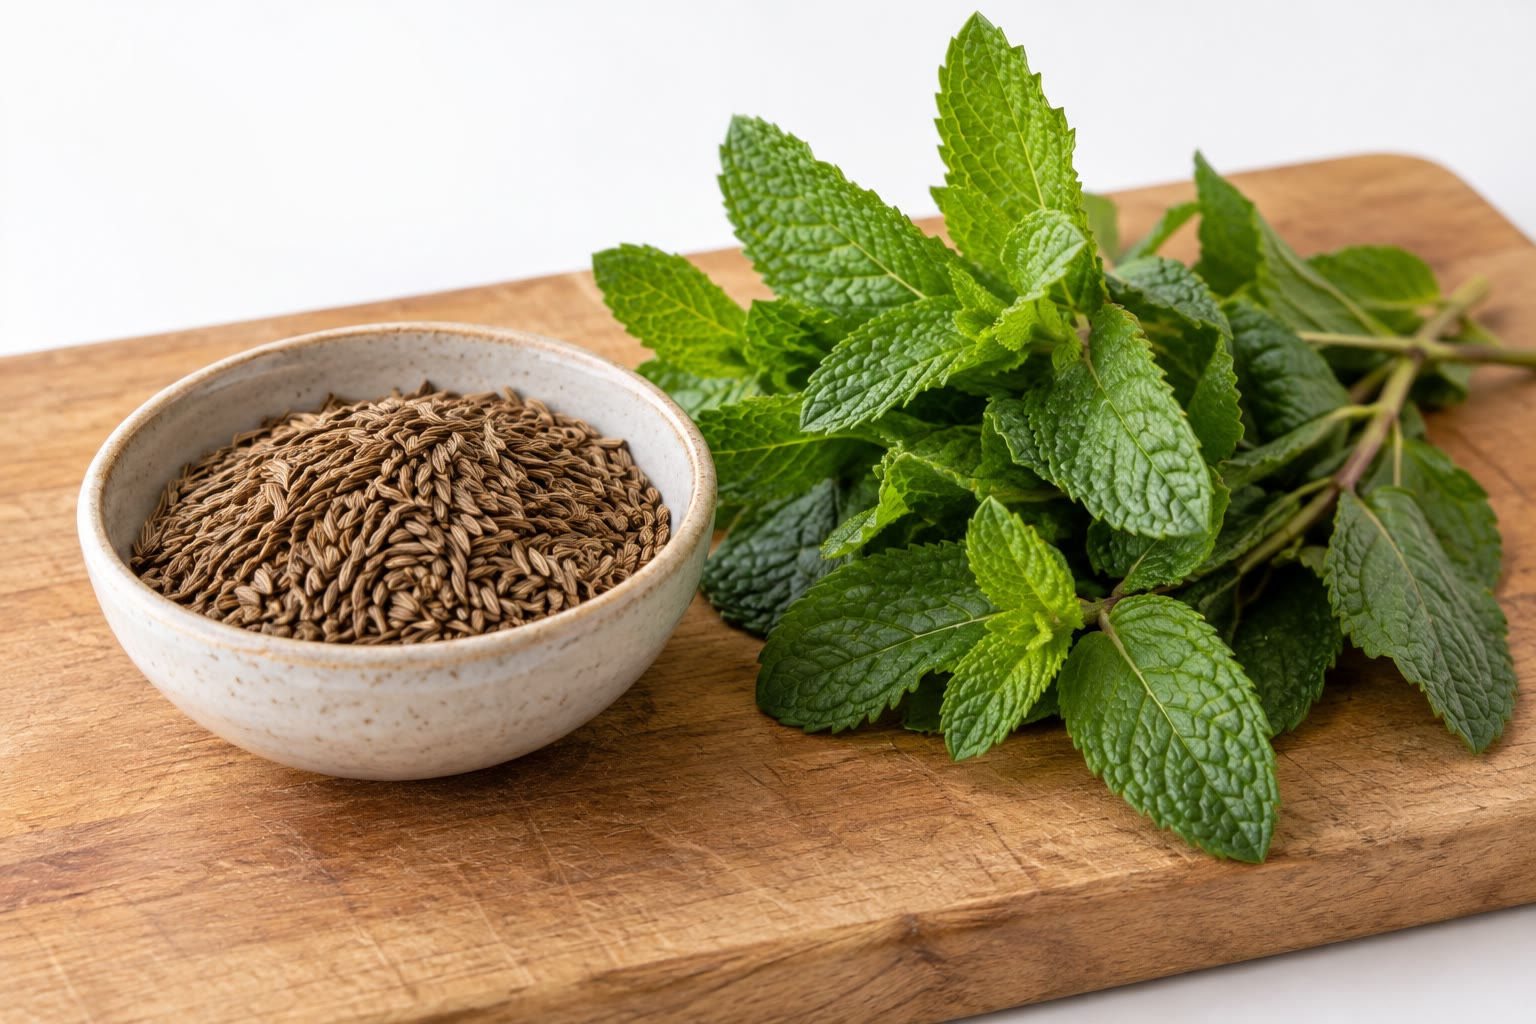
\includegraphics[width=0.55\linewidth]{images/book2/ai/b1-16-caraway-mint.jpg}

{\small Sementes de alcaravia e folhas de hortelã. A alcaravia deve seu
cheiro principalmente à \cip{S}-carvona, a hortelã à sua imagem
especular, a \cip{R}-carvona.}
\end{omfigure}

\section{Isômeros e representações}

\begin{definition}[Constituição, configuração, conformação]\label{def:b1:stereochemistry-in-depth:isomers}
Dois compostos de mesma fórmula cujos átomos estão ligados em ordem
diferente são \emph{isômeros constitucionais}\index{isomeros constitucionais@isômeros constitucionais}.
Compostos de mesma constituição cujos átomos diferem apenas por seu
arranjo no espaço são \emph{estereoisômeros}\index{estereoisomeros@estereoisômeros}. O
arranjo que só pode ser mudado rompendo ligações é a
\emph{configuração}\index{configuracao@configuração} de um estereoisômero; um arranjo obtido
por rotação em torno de ligações simples, sem romper nenhuma, é uma
\emph{conformação}\index{conformacao@conformação}.
\end{definition}

À temperatura ambiente, as rotações em torno das ligações simples
ocorrem bilhões de vezes por segundo: as \omterm{def:b1:stereochemistry-in-depth:isomers}{conformações} se interconvertem
e não podem ser isoladas, enquanto as \omterm{def:b1:stereochemistry-in-depth:isomers}{configurações} são estáveis e dão
compostos distintos.

\begin{definition}[Representações]\label{def:b1:stereochemistry-in-depth:representations}
Na \emph{representação de Cram}\index{representacao de Cram@representação de Cram}, duas ligações
são desenhadas no plano da página, uma cunha cheia aponta para o leitor
e uma cunha tracejada para trás. Uma \emph{projeção de Newman}\index{projecao de Newman@projeção de Newman}
olha a molécula ao longo de uma ligação C--C: o carbono da frente é um
ponto onde se encontram suas três outras ligações, o carbono de trás é
um círculo de cuja borda saem suas ligações. Em uma \emph{projeção de
Fischer}\index{projecao de Fischer@projeção de Fischer}, a cadeia carbônica é vertical, as
ligações horizontais apontam para o leitor e as verticais para trás;
cada cruzamento é um carbono estereogênico.
\end{definition}

\begin{omfigure}
\begin{tikzpicture}[font=\small]
  % staggered and eclipsed ethane, Newman
  \pic (s) at (0,0) {omnewman={90}{30}};
  \foreach \k in {1,2,3} { \node at (s-f\k) {H}; \node at (s-b\k) {H}; }
  \node at (0,-1.9) {alternada};
  \pic (e) at (3.6,0) {omnewman={90}{108}};
  \foreach \k in {1,2,3} { \node at (e-f\k) {H}; }
  \foreach \k in {1,2,3} { \node[font=\scriptsize, black!60] at ($(e-b\k)!-0.12!(e-c)$) {H}; }
  \node at (3.6,-1.9) {eclipsada};
  % Fischer projection of (R)-lactic acid
  \begin{scope}[xshift=7.6cm]
    \draw[thick] (-0.9,0) -- (0.9,0) (0,-0.9) -- (0,0.9);
    \node[above] at (0,0.9) {\ce{COOH}};
    \node[below] at (0,-0.9) {\ce{CH3}};
    \node[left] at (-0.9,0) {H};
    \node[right] at (0.9,0) {OH};
    \node at (0,-1.9) {Fischer};
  \end{scope}
  % Cram of the same
  \begin{scope}[xshift=11.0cm]
    \node at (0,0) {\chemfig{C(-[2]COOH)(-[:210]H_3C)(<:[:-12]OH)(<[:-55]H)}};
    \node at (0,-1.9) {Cram};
  \end{scope}
\end{tikzpicture}

{\small À esquerda: \omterm{def:b1:stereochemistry-in-depth:representations}{projeções de Newman} do etano ao longo de sua ligação
C--C, alternada (ligações de trás entre as da frente) e eclipsada
(ligações de trás escondidas atrás das da frente, desenhadas ligeiramente
deslocadas). À direita: a mesma molécula, o ácido \cip{R}-lático, em
\omterm{def:b1:stereochemistry-in-depth:representations}{projeção de Fischer} e em \omterm{def:b1:stereochemistry-in-depth:representations}{representação de Cram} (as ligações verticais da
cruz de Fischer apontam para trás, as horizontais para o leitor).}
\end{omfigure}

\begin{method}[De Cram para Newman]\label{met:b1:stereochemistry-in-depth:newman-from-cram}
\begin{enumerate}
  \item Escolha a ligação ao longo da qual olhar e a extremidade mais
        próxima do olho.
  \item Desenhe as três ligações do carbono da frente a partir do centro,
        conservando sua ordem (sentido horário ou anti-horário) vista do
        olho.
  \item Desenhe as ligações do carbono de trás a partir do círculo, com a
        ordem vista do mesmo lado.
  \item Verifique: girar o carbono de trás de $60^\circ$ passa de
        alternada a eclipsada; de $120^\circ$, de uma \omterm{def:b1:stereochemistry-in-depth:conformations}{conformação
        alternada} à seguinte.
\end{enumerate}
\end{method}

\section{A configuração: as regras CIP}

\begin{definition}[Regras CIP, descritores]\label{def:b1:stereochemistry-in-depth:cip}
As \emph{regras CIP}\index{regras CIP} (Cahn--Ingold--Prelog) ordenam os
quatro substituintes de um \omterm{def:b1:stereochemistry-in-depth:stereocentre}{centro estereogênico}: maior número atômico
primeiro; em caso de empate, comparam-se os conjuntos de átomos ligados
em seguida, e assim por diante, para fora; uma ligação dupla conta como
duas ligações simples a átomos duplicados. Com o substituinte de menor
prioridade apontando para longe do olho, a sequência $1 \to 2 \to 3$ no
sentido horário define o descritor \cip{R}, e no sentido anti-horário,
\cip{S}. Para uma ligação dupla com dois substituintes em cada carbono,
\cip{Z} significa que os dois de maior prioridade estão do mesmo lado, e
\cip{E}, em lados opostos.
\end{definition}

\begin{method}[Atribuir \texorpdfstring{\cip{R}}{(R)} ou \texorpdfstring{\cip{S}}{(S)}]\label{met:b1:stereochemistry-in-depth:cip}
\begin{enumerate}
  \item Ordene os quatro substituintes pelas \omterm{def:b1:stereochemistry-in-depth:cip}{regras CIP}.
  \item Se o de menor prioridade aponta para longe de você (cunha
        tracejada, ou ligação vertical de uma \omterm{def:b1:stereochemistry-in-depth:representations}{projeção de Fischer}), leia
        diretamente o sentido de $1 \to 2 \to 3$.
  \item Se ele aponta para você (cunha cheia, ligação horizontal de
        Fischer), leia o sentido e inverta o descritor.
  \item Trocar dois substituintes quaisquer inverte o descritor: uma
        verificação rápida.
\end{enumerate}
No ácido lático, $\ce{OH} > \ce{COOH} > \ce{CH3} > \ce{H}$ (O; depois
C(O,O,O) vence C(H,H,H)). Na \omterm{def:b1:stereochemistry-in-depth:representations}{projeção de Fischer} acima, H está na
horizontal (para nós) e $\ce{OH} \to \ce{COOH} \to \ce{CH3}$ gira no
sentido anti-horário: invertido, o centro é \cip{R}.
\end{method}

\section{A quiralidade e suas consequências}

\begin{definition}[Centro estereogênico, quiralidade]\label{def:b1:stereochemistry-in-depth:stereocentre}
Um objeto é \emph{quiral}\index{quiral} se não pode ser sobreposto à
sua imagem especular, e \emph{aquiral}\index{aquiral} caso contrário; a
propriedade é a \emph{quiralidade}\index{quiralidade}. Um \emph{centro
estereogênico}\index{centro estereogenico@centro estereogênico} é um átomo no qual a troca de dois
substituintes dá um \omterm{def:b1:stereochemistry-in-depth:isomers}{estereoisômero}; um carbono tetraédrico com quatro
substituintes diferentes é um deles.
\end{definition}

Uma molécula com um plano de simetria ou um centro de simetria é
\omterm{def:b1:stereochemistry-in-depth:stereocentre}{aquiral}; uma molécula sem nenhum dos dois é, na prática, \omterm{def:b1:stereochemistry-in-depth:stereocentre}{quiral}. O
critério exato, em termos de operações de simetria, é dado no volume do
3.º~ano.

\begin{definition}[Enantiômeros, diastereoisômeros, composto meso, mistura racêmica]\label{def:b1:stereochemistry-in-depth:enantiomers}
Dois \omterm{def:b1:stereochemistry-in-depth:isomers}{estereoisômeros} que são imagens especulares um do outro são
\emph{enantiômeros}\index{enantiomeros@enantiômeros}; \omterm{def:b1:stereochemistry-in-depth:isomers}{estereoisômeros} que não o são são
\emph{diastereoisômeros}\index{diastereoisomeros@diastereoisômeros}. Um \emph{composto
meso}\index{composto meso} tem \omterm{def:b1:stereochemistry-in-depth:stereocentre}{centros estereogênicos}, mas é \omterm{def:b1:stereochemistry-in-depth:stereocentre}{aquiral}. Uma
mistura equimolar de dois enantiômeros é uma \emph{mistura
racêmica}\index{mistura racemica@mistura racêmica}.
\end{definition}

\begin{proposition}[Número de estereoisômeros]\label{prop:b1:stereochemistry-in-depth:max-stereoisomers}
Uma molécula com $n$ \omterm{def:b1:stereochemistry-in-depth:stereocentre}{centros estereogênicos} (e nenhuma outra unidade
estereogênica) tem no máximo $2^n$ \omterm{def:b1:stereochemistry-in-depth:isomers}{estereoisômeros}, em no máximo
$2^{n-1}$ pares de \omterm{def:b1:stereochemistry-in-depth:enantiomers}{enantiômeros}; as formas meso diminuem esse número.
\end{proposition}

\begin{proof}
Cada centro é \cip{R} ou \cip{S} independentemente: $2^n$ combinações. A
imagem especular muda todos os descritores, de modo que as combinações
se agrupam em pares de \omterm{def:b1:stereochemistry-in-depth:enantiomers}{enantiômeros}, $2^{n-1}$ pares. Se uma combinação
é sua própria imagem especular após uma rotação da molécula (uma forma
meso), seu par se reduz a um único composto.
\end{proof}

O ácido tartárico, \ce{HOOC-CH(OH)-CH(OH)-COOH}, tem dois centros
equivalentes: \cip{R,R} e \cip{S,S} são \omterm{def:b1:stereochemistry-in-depth:enantiomers}{enantiômeros}, enquanto \cip{R,S}
tem um plano especular entre os dois carbonos e é meso: três
\omterm{def:b1:stereochemistry-in-depth:isomers}{estereoisômeros}, e não quatro.

\begin{proposition}[Propriedades dos enantiômeros]\label{prop:b1:stereochemistry-in-depth:enantiomer-properties}
Dois \omterm{def:b1:stereochemistry-in-depth:enantiomers}{enantiômeros} têm as mesmas temperaturas de fusão e de ebulição, as
mesmas \omterm{def:b1:precipitation:solubility}{solubilidades} em solventes \omterm{def:b1:stereochemistry-in-depth:stereocentre}{aquirais}, os mesmos espectros e a
mesma reatividade diante de reagentes \omterm{def:b1:stereochemistry-in-depth:stereocentre}{aquirais}; eles diferem por sua
ação sobre a luz polarizada e por suas interações com outras moléculas
\omterm{def:b1:stereochemistry-in-depth:stereocentre}{quirais}. Os \omterm{def:b1:stereochemistry-in-depth:enantiomers}{diastereoisômeros} diferem em todas as suas propriedades.
\end{proposition}

\begin{proof}
Toda propriedade que só depende de distâncias e ângulos dentro da
molécula, ou entre ela e parceiros \omterm{def:b1:stereochemistry-in-depth:stereocentre}{aquirais}, é a mesma para um objeto e
sua imagem especular, já que uma reflexão conserva distâncias e ângulos.
Um parceiro \omterm{def:b1:stereochemistry-in-depth:stereocentre}{quiral} (um receptor, um reagente \omterm{def:b1:stereochemistry-in-depth:stereocentre}{quiral}, o percurso
helicoidal da luz polarizada descrito adiante) forma pares
diastereoisoméricos, que já não são imagens especulares e, portanto,
diferem. Os \omterm{def:b1:stereochemistry-in-depth:enantiomers}{diastereoisômeros} não estão relacionados por nenhuma
reflexão: suas distâncias internas diferem.
\end{proof}

\begin{omfigure}
\begin{tikzpicture}[font=\small, line join=round]
  \foreach \dx/\kind/\lab in {0/1/{\cip{R}-carvona (hortelã)}, 5.2/0/{\cip{S}-carvona (alcaravia)}} {
  \begin{scope}[xshift=\dx cm]
    \coordinate (c1) at (0,1); \coordinate (c2) at (0.87,0.5);
    \coordinate (c3) at (0.87,-0.5); \coordinate (c4) at (0,-1);
    \coordinate (c5) at (-0.87,-0.5); \coordinate (c6) at (-0.87,0.5);
    \draw[thick] (c1) -- (c2) -- (c3) -- (c4) -- (c5) -- (c6) -- cycle;
    \draw[thick] ($(c2)!0.15!(c3)+(-0.12,0)$) -- ($(c3)!0.15!(c2)+(-0.12,0)$);
    \draw[thick] (c1) -- ++(0,0.7) node[above] {O};
    \draw[thick] ($(c1)+(0.1,0)$) -- ++(0,0.62);
    \draw[thick] (c2) -- ++(0.75,0.43) node[right] {\ce{CH3}};
    \coordinate (q) at ($(c5)+(-0.75,-0.43)$);
    \ifnum\kind=1
      \fill (c5) -- ($(q)+(0.06,-0.1)$) -- ($(q)+(-0.06,0.1)$) -- cycle;
    \else
      \foreach \t in {0.15,0.3,0.45,0.6,0.75,0.9}
        \draw ($(c5)!\t!(q)+(\t*0.06,-\t*0.1)$) -- ($(c5)!\t!(q)+(-\t*0.06,\t*0.1)$);
    \fi
    \draw[thick] (q) -- ++(-0.6,0.5) node[above] {\ce{CH2}};
    \draw[thick] ($(q)+(0.08,0.06)$) -- ++(-0.6,0.5);
    \draw[thick] (q) -- ++(0,-0.75) node[below] {\ce{CH3}};
    \node[font=\scriptsize] at ($(c5)+(0.35,0.12)$) {5};
    \node at (0,-2.85) {\lab};
  \end{scope}}
\end{tikzpicture}

{\small As duas carvonas, desenhadas sobre o mesmo esqueleto: o grupo
isopropenila em C5 aponta para o leitor (cunha cheia) em uma e para trás
(cunha tracejada) na outra, com o hidrogênio de C5 (não desenhado) do
lado oposto. Elas são imagens especulares uma da outra: \omterm{def:b1:stereochemistry-in-depth:enantiomers}{enantiômeros}
(\cref{exo:b1:stereochemistry-in-depth:4}).}
\end{omfigure}

\begin{history}[Um carbono tetraédrico]
\begin{minipage}[t]{0.2\linewidth}\vspace{0pt}
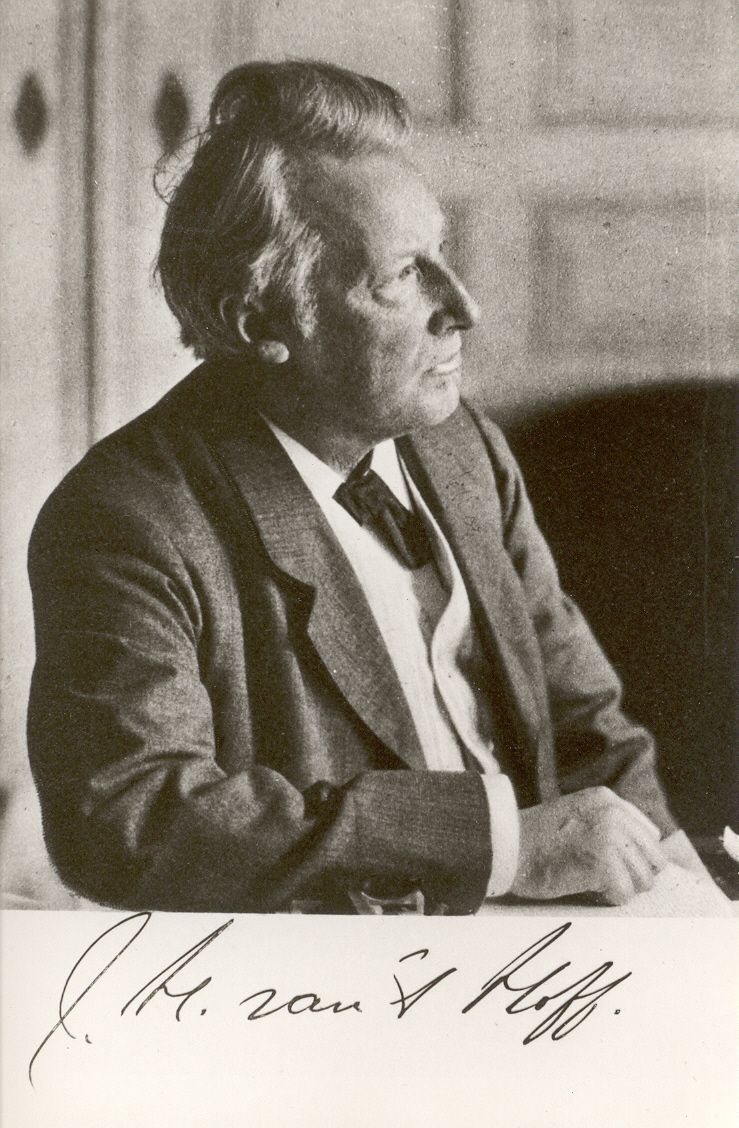
\includegraphics[width=\linewidth]{images/book2/van-t-hoff.jpg}
\end{minipage}\hfill
\begin{minipage}[t]{0.76\linewidth}\vspace{0pt}
Jacobus Henricus van 't Hoff propôs, ainda jovem químico, que as quatro
ligações de um átomo de carbono apontam para os vértices de um
tetraedro. Um carbono com quatro substituintes diferentes existe então
em dois arranjos que são imagens especulares, o que explicava por que
certos compostos se apresentam em duas formas que só diferem pela
maneira como giram a luz polarizada. A ideia é o ponto de partida de
todos os desenhos deste capítulo.
(Fotografia publicada em 1911, domínio público, Wikimedia Commons.)
\end{minipage}
\end{history}

\section{Conformações}

\begin{definition}[Ângulo de torção e conformações]\label{def:b1:stereochemistry-in-depth:conformations}
Para quatro átomos A--B--C--D, o \emph{ângulo de torção}\index{angulo de torcao@ângulo de torção}
$\theta$ em torno de B--C é o ângulo entre os planos ABC e BCD, lido em
uma \omterm{def:b1:stereochemistry-in-depth:representations}{projeção de Newman} ao longo de B--C. Uma \omterm{def:b1:stereochemistry-in-depth:isomers}{conformação} é uma
\emph{conformação eclipsada}\index{conformacao eclipsada@conformação eclipsada} quando as ligações
dos carbonos da frente e de trás estão alinhadas em projeção, e uma
\emph{conformação alternada}\index{conformacao alternada@conformação alternada} quando elas se
alternam. No butano, visto ao longo de C2--C3, a \omterm{def:b1:stereochemistry-in-depth:isomers}{conformação} alternada
com os dois grupos metila a $180^\circ$ é a \emph{conformação anti}\index{conformacao anti@conformação anti},
e as que os têm a $\pm 60^\circ$ são as \emph{conformações
gauche}\index{conformacao gauche@conformação gauche}. No ciclo-hexano, o anel pregueado sem
tensão é a \emph{cadeira}\index{cadeira}; cada carbono leva uma ligação
\emph{axial}\index{axial}, paralela ao eixo do anel, e uma ligação
\emph{equatorial}\index{equatorial}, aproximadamente no plano médio do
anel. A \emph{inversão do anel}\index{inversao do anel@inversão do anel} converte uma
cadeira na outra, com toda ligação axial tornando-se equatorial e
vice-versa.
\end{definition}

\begin{omfigure}
\begin{tikzpicture}
\begin{axis}[
  width=0.82\linewidth, height=5.8cm, xmin=0, xmax=360, ymin=0, ymax=21,
  legend style={font=\scriptsize, draw=none, at={(0.5,0.62)}, anchor=center},
  axis x line=bottom, axis y line=left, xlabel={ângulo de torção $\theta$ (graus)},
  ylabel={energia (kJ/mol)}, xtick={0,60,120,180,240,300,360},
  tick label style={font=\small}, label style={font=\small}]
\addplot[omDef, very thick] table[x=theta, y=butane] {figdata/out/bachelor-1-butane-torsion.dat};
\addplot[omProp, thick, dashed] table[x=theta, y=ethane] {figdata/out/bachelor-1-butane-torsion.dat};
\node[font=\scriptsize, anchor=south west] at (axis cs:0,18.4) {syn};
\node[font=\scriptsize, anchor=south] at (axis cs:62,18.4) {gauche};
\node[font=\scriptsize, anchor=south] at (axis cs:120,18.4) {eclipsada};
\node[font=\scriptsize, anchor=south] at (axis cs:180,18.4) {anti};
\node[font=\scriptsize, anchor=south] at (axis cs:240,18.4) {eclipsada};
\node[font=\scriptsize, anchor=south] at (axis cs:298,18.4) {gauche};
\node[font=\scriptsize, anchor=south east] at (axis cs:360,18.4) {syn};
\legend{butano, etano}
\end{axis}
\end{tikzpicture}

{\small Energia de torção do butano em torno de sua ligação central
(linha cheia; $\theta
= 0$ quando os grupos metila se eclipsam) e do etano (tracejada),
calculada a partir de potenciais de torção experimentais. Etano: barreira
de \qty{12.2}{kJ/mol}. Butano: anti é a mais estável; gauche, \qty{2.8}{kJ/mol}
acima, em $\theta = 62^\circ$; barreiras de \qty{15.2}{kJ/mol} (metila
eclipsando hidrogênio) e \qty{16.5}{kJ/mol} (metila eclipsando metila).}
% ledger: rot:ethane-V3, rot:butane-V1, rot:butane-V2, rot:butane-V3, rot:butane-V4, rot:butane-V5, rot:butane-V6 (curves in figdata/bachelor-1/butane-torsion.py)
\end{omfigure}

As barreiras são pequenas diante da energia térmica disponível nas
colisões ($RT = \qty{2.5}{kJ/mol}$ à temperatura ambiente, e muito mais
na cauda da distribuição, \cref{ch:b1:elementary-steps}): a rotação é
rápida, e o butano é uma mistura de moléculas anti e gauche que não podem
ser separadas.

\begin{method}[Desenhar uma cadeira]\label{met:b1:stereochemistry-in-depth:draw-chair}
\begin{enumerate}
  \item Desenhe duas linhas paralelas levemente inclinadas para baixo à
        direita, deslocadas; una suas extremidades com um V à esquerda e
        um V invertido à direita para fechar o anel de seis membros.
  \item As ligações \omterm{def:b1:stereochemistry-in-depth:conformations}{axiais} são verticais: para cima nos carbonos que
        apontam para cima, para baixo nos que apontam para baixo,
        alternando ao longo do anel.
  \item As ligações \omterm{def:b1:stereochemistry-in-depth:conformations}{equatoriais} são paralelas às ligações do anel
        situadas uma posição adiante e apontam para fora.
  \item Para inverter o anel, desenhe a outra \omterm{def:b1:stereochemistry-in-depth:conformations}{cadeira}; um substituinte
        \omterm{def:b1:stereochemistry-in-depth:conformations}{axial} em uma é \omterm{def:b1:stereochemistry-in-depth:conformations}{equatorial} na outra.
\end{enumerate}
\end{method}

\begin{omfigure}
\begin{tikzpicture}[font=\small]
  \pic (a) at (0,0) {omchair};
  \foreach \k in {1,2,3,4,5,6} \draw[omProp, thick] (a-c\k) -- (a-a\k);
  \foreach \k in {1,2,3,4,5,6} \draw[omDef, thick] (a-c\k) -- (a-e\k);
  \node[omProp, anchor=south] at (a-a3) {axial};
  \node[omDef, anchor=north] at (a-e5) {equatorial};
  \begin{scope}[xshift=4.9cm]
    \pic (b) at (0,0) {omchair};
    \draw[thick] (b-c1) -- (b-e1) node[right] {\ce{CH3}};
    \draw[thick] (b-c1) -- (b-a1) node[above] {H};
    \node at (0,-1.5) {\ce{CH3} equatorial};
  \end{scope}
  \draw[<->, thick] (8.1,0) -- (8.8,0) node[midway, above] {\scriptsize\raisebox{0.8ex}{inversão}};
  \begin{scope}[xshift=10.45cm]
    \pic (c) at (0,0) {omchairflip};
    \draw[thick] (c-c4) -- (c-a4) node[below] {\ce{CH3}};
    \draw[thick] (c-c4) -- (c-e4) node[right] {H};
    \node at (0,-1.5) {\ce{CH3} axial};
  \end{scope}
\end{tikzpicture}

{\small À esquerda: a \omterm{def:b1:stereochemistry-in-depth:conformations}{cadeira} do ciclo-hexano com suas seis ligações
\omterm{def:b1:stereochemistry-in-depth:conformations}{axiais} (em laranja, alternadamente para cima e para baixo) e suas seis
ligações \omterm{def:b1:stereochemistry-in-depth:conformations}{equatoriais} (em azul). À direita: as duas \omterm{def:b1:stereochemistry-in-depth:conformations}{cadeiras} do
metilciclo-hexano, interconvertidas pela \omterm{def:b1:stereochemistry-in-depth:conformations}{inversão do anel}; o grupo
metila é \omterm{def:b1:stereochemistry-in-depth:conformations}{equatorial} em uma e \omterm{def:b1:stereochemistry-in-depth:conformations}{axial} na outra.}
\end{omfigure}

\begin{proposition}[Os substituintes equatoriais são preferidos]\label{prop:b1:stereochemistry-in-depth:chair-substituent}
Em um ciclo-hexano monossubstituído, a \omterm{def:b1:stereochemistry-in-depth:conformations}{cadeira} com o substituinte
\omterm{def:b1:stereochemistry-in-depth:conformations}{equatorial} é a mais estável. Para um grupo metila, a posição \omterm{def:b1:stereochemistry-in-depth:conformations}{axial}
acrescenta duas interações gauche com carbonos do anel, cada uma valendo
a do butano (\qtyrange{2.8}{2.9}{kJ/mol}), cerca de \qty{5.7}{kJ/mol} no
total: uma estimativa da diferença de energia.
\end{proposition}

\begin{proof}
Visto ao longo da ligação C1--C2, um metila \omterm{def:b1:stereochemistry-in-depth:conformations}{axial} em C1 está em gauche
com C3 do anel; visto ao longo de C1--C6, em gauche com C5: duas
interações gauche do tipo butano, que também se veem como a aglomeração
do metila com os hidrogênios \omterm{def:b1:stereochemistry-in-depth:conformations}{axiais} de C3 e C5 (as interações
1,3-diaxiais). Um metila \omterm{def:b1:stereochemistry-in-depth:conformations}{equatorial} está em anti com C3 e C5. Cada
interação gauche custa o que custa no butano, \qty{2.8}{kJ/mol} no
potencial de torção da figura.
\end{proof}

Com $\Delta E = \qty{5.7}{kJ/mol}$, a razão entre \omterm{def:b1:stereochemistry-in-depth:conformations}{cadeiras} \omterm{def:b1:stereochemistry-in-depth:conformations}{equatoriais} e
\omterm{def:b1:stereochemistry-in-depth:conformations}{axiais} a \qty{25}{\celsius} é $\exp(\Delta E/RT) = 10$: cerca de
\qty{91}{\percent} \omterm{def:b1:stereochemistry-in-depth:conformations}{equatoriais} (\cref{exo:b1:stereochemistry-in-depth:9}).
Grupos grandes, como o terc-butila, travam o anel na \omterm{def:b1:stereochemistry-in-depth:conformations}{cadeira} em que
ficam \omterm{def:b1:stereochemistry-in-depth:conformations}{equatoriais}.

\section{Atividade óptica}

\begin{definition}[Atividade óptica, poder rotatório específico]\label{def:b1:stereochemistry-in-depth:optical-activity}
Uma substância apresenta \emph{atividade óptica}\index{atividade optica@atividade óptica} se gira
o plano de polarização da luz linearmente polarizada que a atravessa.
Para um observador voltado para a luz, uma substância
\emph{dextrogira}\index{dextrogira}, indicada por $(+)$, o gira no
sentido horário, e uma substância \emph{levogira}\index{levogira},
$(-)$, no sentido anti-horário. O \emph{poder rotatório
específico}\index{poder rotatorio especifico@poder rotatório específico} é $[\alpha] = \alpha/(\ell c)$, em que
$\alpha$ é o ângulo medido em graus, $\ell$ o comprimento do percurso em
decímetros e $c$ a concentração mássica em \unit{g/mL}; ele depende do
comprimento de onda (em geral a raia amarela do sódio), da temperatura e
do solvente.
\end{definition}

\begin{omfigure}
\begin{tikzpicture}[font=\small, >={Stealth}]
  \fill[yellow!70!orange] (0,0) circle (0.25);
  \node[below] at (0,-0.45) {lâmpada};
  \draw[thick] (1.3,-0.7) rectangle (1.45,0.7); \node[below] at (1.37,-0.75) {polarizador};
  \draw[omDef!20, fill=omDef!10] (2.4,-0.45) rectangle (5.6,0.45);
  \node at (4.0,0) {\scriptsize amostra, comprimento $\ell$};
  \draw[thick] (6.5,-0.7) rectangle (6.65,0.7); \node[below] at (6.57,-0.75) {analisador};
  \draw (7.6,0) circle (0.3); \node[below] at (7.6,-0.45) {olho};
  \draw[->, orange!80!black] (0.3,0) -- (1.25,0);
  \draw[->, orange!80!black] (1.5,0) -- (2.35,0);
  \draw[->, orange!80!black] (5.65,0) -- (6.45,0);
  % polarisation planes
  \draw[thick, omThm] (1.9,-0.35) -- (1.9,0.35);
  \draw[thick, omThm] (6.05,-0.33) -- ++(70:0.0) -- (5.93,0.33);
  \draw[->, omThm] (5.75,0.55) arc[start angle=100, end angle=70, radius=0.6];
  \node[omThm, above] at (6.1,0.75) {$\alpha$};
\end{tikzpicture}

{\small Um polarímetro. O polarizador deixa passar a luz que vibra em um
plano; a amostra \omterm{def:b1:stereochemistry-in-depth:stereocentre}{quiral} gira esse plano de $\alpha$; o analisador é
girado até que a luz se extinga de novo, o que mede $\alpha$.}
\end{omfigure}

\begin{proposition}[Lei de Biot]\label{prop:b1:stereochemistry-in-depth:biot}
Para uma solução diluída de vários solutos opticamente ativos, o ângulo
de rotação é aditivo, $\alpha = \ell\sum_i [\alpha]_i c_i$ (\emph{lei de
Biot}\index{lei de Biot}). Dois \omterm{def:b1:stereochemistry-in-depth:enantiomers}{enantiômeros} têm \omterm{def:b1:stereochemistry-in-depth:optical-activity}{poderes rotatórios
específicos} opostos; uma \omterm{def:b1:stereochemistry-in-depth:enantiomers}{mistura racêmica} não gira a luz.
\end{proposition}

\begin{proof}
Cada soluto contribui independentemente em solução diluída, em
proporção ao número de moléculas atravessadas, isto é, a $\ell c_i$;
esse é o conteúdo experimental da lei. Uma reflexão troca o sentido
horário pelo anti-horário: a molécula imagem especular gira o plano do
ângulo oposto, e em uma \omterm{def:b1:stereochemistry-in-depth:enantiomers}{mistura racêmica} as duas contribuições se
anulam.
\end{proof}

Para uma mistura de dois \omterm{def:b1:stereochemistry-in-depth:enantiomers}{enantiômeros} de concentração total $c$, a
fração $x$ da forma $(-)$ dá $\alpha = \ell c[\alpha]_{(-)}(x - (1 - x)) =
\ell c[\alpha]_{(-)}(2x - 1)$: medir $\alpha$ dá a composição. A rotação
óptica não está ligada de nenhuma maneira simples ao descritor: um
composto \cip{R} pode ser $(+)$ ou $(-)$; a \cip{R}-carvona da hortelã é
\omterm{def:b1:stereochemistry-in-depth:optical-activity}{levogira}.

\section{Exercícios}

\begin{exercise}[$\star$]\label{exo:b1:stereochemistry-in-depth:1}
Classifique cada par como \omterm{def:b1:stereochemistry-in-depth:isomers}{isômeros constitucionais}, \omterm{def:b1:stereochemistry-in-depth:enantiomers}{enantiômeros},
\omterm{def:b1:stereochemistry-in-depth:enantiomers}{diastereoisômeros} ou duas \omterm{def:b1:stereochemistry-in-depth:isomers}{conformações} de um mesmo composto: butan-1-ol
e butan-2-ol; \cip{R}- e \cip{S}-butan-2-ol; \cip{Z}- e
\cip{E}-but-2-eno; as \omterm{def:b1:stereochemistry-in-depth:isomers}{conformações} anti e gauche do butano; ácido
\cip{R,R}- e \cip{R,S}-tartárico.
\end{exercise}

\begin{exercise}[$\star$]\label{exo:b1:stereochemistry-in-depth:2}
Ordene pelas \omterm{def:b1:stereochemistry-in-depth:cip}{regras CIP}: \ce{-OH}, \ce{-NH2}, \ce{-CH3}, \ce{-H}; depois
\ce{-CH2OH}, \ce{-CHO}, \ce{-COOH}, \ce{-CH(CH3)2}; depois \ce{-Cl},
\ce{-CH2Cl}, \ce{-CCl3}, \ce{-Br}.
\end{exercise}

\begin{exercise}[$\star$]\label{exo:b1:stereochemistry-in-depth:3}
Quantos \omterm{def:b1:stereochemistry-in-depth:isomers}{estereoisômeros} têm o 2,3-diclorobutano, o
2-bromo-3-clorobutano e o pentano-2,4-diol? Identifique as formas meso.
\end{exercise}

\begin{exercise}[$\star$]\label{exo:b1:stereochemistry-in-depth:4}
Ordene pelas \omterm{def:b1:stereochemistry-in-depth:cip}{regras CIP} os quatro substituintes de C5 da carvona e
verifique os descritores dados na figura das duas carvonas (cunha cheia:
o grupo isopropenila voltado para o leitor, H para trás).
\end{exercise}

\begin{exercise}[$\star\star$]\label{exo:b1:stereochemistry-in-depth:5}
Desenhe as \omterm{def:b1:stereochemistry-in-depth:representations}{projeções de Newman} do butano ao longo de C2--C3 em
$\theta = 0$, 60, 120 e $180^\circ$ e leia suas energias na curva. Que
fração das moléculas seria gauche se as energias gauche e anti fossem
iguais?
\end{exercise}

\begin{exercise}[$\star\star$]\label{exo:b1:stereochemistry-in-depth:6}
Desenhe a \omterm{def:b1:stereochemistry-in-depth:representations}{projeção de Fischer} da \cip{S}-alanina,
\ce{H2N-CH(CH3)-COOH}, com o grupo ácido no alto. De que lado fica o
grupo amino?
\end{exercise}

\begin{exercise}[$\star\star$]\label{exo:b1:stereochemistry-in-depth:7}
Mostre que o \textit{cis}-1,2-dimetilciclo-hexano tem um metila \omterm{def:b1:stereochemistry-in-depth:conformations}{axial} e
um \omterm{def:b1:stereochemistry-in-depth:conformations}{equatorial} nas duas \omterm{def:b1:stereochemistry-in-depth:conformations}{cadeiras}, enquanto o isômero \textit{trans} tem
uma \omterm{def:b1:stereochemistry-in-depth:conformations}{cadeira} com os dois \omterm{def:b1:stereochemistry-in-depth:conformations}{equatoriais}. Qual isômero é mais estável? Use a
estimativa do capítulo.
\end{exercise}

\begin{exercise}[$\star\star$]\label{exo:b1:stereochemistry-in-depth:8}
Uma solução de um composto \omterm{def:b1:stereochemistry-in-depth:stereocentre}{quiral} a \qty{0.100}{g/mL} em um tubo de
\qty{2.00}{dm} gira a luz de $+13.2^\circ$. Calcule $[\alpha]$. O que
daria um tubo de \qty{1.00}{dm}? E o \omterm{def:b1:stereochemistry-in-depth:enantiomers}{enantiômero} na mesma concentração?
\end{exercise}

\begin{exercise}[$\star\star$]\label{exo:b1:stereochemistry-in-depth:9}
Calcule, com $\Delta E = \qty{5.7}{kJ/mol}$ e a razão de Boltzmann
$\exp(\Delta E/RT)$, a fração de \omterm{def:b1:stereochemistry-in-depth:conformations}{cadeiras} do metilciclo-hexano com o
metila \omterm{def:b1:stereochemistry-in-depth:conformations}{equatorial} a \qty{25}{\celsius} e a \qty{-50}{\celsius}.
\end{exercise}

\begin{exercise}[$\star\star\star$]\label{exo:b1:stereochemistry-in-depth:10}
Explique por que o etano tem um único tipo de \omterm{def:b1:stereochemistry-in-depth:conformations}{conformação alternada} e o
butano dois (anti e gauche), e por que a gauche é menos estável. Usando
as energias da figura, estime a razão de populações anti : gauche do
butano a \qty{25}{\celsius} (duas \omterm{def:b1:stereochemistry-in-depth:conformations}{conformações gauche}, uma anti).
\end{exercise}

\begin{exercise}[$\star\star\star$]\label{exo:b1:stereochemistry-in-depth:11}
Considere o ácido 2,3,4-tri-hidroxipentanodioico,
\ce{HOOC-CH(OH)-CH(OH)-CH(OH)-COOH}. Conte seus \omterm{def:b1:stereochemistry-in-depth:stereocentre}{centros estereogênicos},
mostre que o carbono central só é estereogênico quando os dois externos
têm descritores opostos (pseudoassimétrico) e conte os \omterm{def:b1:stereochemistry-in-depth:isomers}{estereoisômeros}
(meso incluídos).
\end{exercise}

\begin{exercise}[$\star\star\star$]\label{exo:b1:stereochemistry-in-depth:12}
Uma amostra de um \omterm{def:b1:stereochemistry-in-depth:enantiomers}{enantiômero} de um composto ($[\alpha] = +66.0^\circ$
para o composto puro nas condições usadas) sofreu racemização parcial: a
\qty{0.050}{g/mL} em um tubo de \qty{1.00}{dm}, ela dá $+2.31^\circ$.
Calcule as frações dos dois \omterm{def:b1:stereochemistry-in-depth:enantiomers}{enantiômeros}.
\end{exercise}

\section{Problema: O mentol, a molécula refrescante}

\begin{problem}[{Problema de fim de semana --- os três estereocentros do
mentol, seus oito estereoisômeros, a cadeira toda equatorial, a lei de
Biot e a porcentagem de (\textminus)-mentol em uma amostra parcialmente
racemizada}]
\label{pb:b1:stereochemistry-in-depth:1}
O mentol, 2-isopropil-5-metilciclo-hexan-1-ol, dá à hortelã sua sensação
refrescante. O composto natural é o $(-)$-mentol, de \omterm{def:b1:stereochemistry-in-depth:isomers}{configuração}
\cip{1R,2S,5R}. Um laboratório mede com um polarímetro (raia do sódio,
\qty{25}{\celsius}, etanol, $\ell = \qty{1.00}{dm}$): sua amostra de
referência de $(-)$-mentol puro a $c = \qty{0.0500}{g/mL}$ dá $\alpha =
-2.46^\circ$; uma amostra a testar, na mesma concentração, dá
$-1.97^\circ$.

\medskip
\noindent\textbf{Parte I --- Estereocentros.}
\begin{enumerate}
  \item Desenhe a constituição do mentol e marque os carbonos
        estereogênicos.
  \item Quantos \omterm{def:b1:stereochemistry-in-depth:isomers}{estereoisômeros} pode haver? Quantos pares de
        \omterm{def:b1:stereochemistry-in-depth:enantiomers}{enantiômeros}?
  \item Por que não há forma meso?
  \item Ordene os substituintes de C1 pelas \omterm{def:b1:stereochemistry-in-depth:cip}{regras CIP}.
  \item Ordene os substituintes de C2.
  \item Ordene os substituintes de C5.
  \item Escreva a \omterm{def:b1:stereochemistry-in-depth:isomers}{configuração} do \omterm{def:b1:stereochemistry-in-depth:enantiomers}{enantiômero} do $(-)$-mentol.
\end{enumerate}

\medskip
\noindent\textbf{Parte II --- A \omterm{def:b1:stereochemistry-in-depth:conformations}{cadeira}.}
\begin{enumerate}[resume]
  \item Desenhe uma \omterm{def:b1:stereochemistry-in-depth:conformations}{cadeira} de ciclo-hexano e coloque os três
        substituintes do $(-)$-mentol todos \omterm{def:b1:stereochemistry-in-depth:conformations}{equatoriais}. Verifique que isso
        corresponde ao arranjo relativo (1,2-\textit{trans} e
        1,5-\textit{cis}) do mentol.
  \item O que acontece com os três substituintes na \omterm{def:b1:stereochemistry-in-depth:conformations}{cadeira} invertida?
  \item Usando a estimativa do capítulo para um metila \omterm{def:b1:stereochemistry-in-depth:conformations}{axial}, explique
        por que o mentol está quase inteiramente em uma única \omterm{def:b1:stereochemistry-in-depth:conformations}{cadeira}.
  \item O neomentol difere do mentol apenas em C1. Ele é um \omterm{def:b1:stereochemistry-in-depth:enantiomers}{enantiômero} ou
        um \omterm{def:b1:stereochemistry-in-depth:enantiomers}{diastereoisômero} do mentol?
  \item Na melhor \omterm{def:b1:stereochemistry-in-depth:conformations}{cadeira} do neomentol, que grupo é \omterm{def:b1:stereochemistry-in-depth:conformations}{axial}?
  \item Por que o mentol e o neomentol têm temperaturas de ebulição
        diferentes, enquanto os dois \omterm{def:b1:stereochemistry-in-depth:enantiomers}{enantiômeros} do mentol não têm?
\end{enumerate}

\medskip
\noindent\textbf{Parte III --- A rotação óptica.}
\begin{enumerate}[resume]
  \item Calcule $[\alpha]$ da amostra de referência. Compare com o
        intervalo de $-45^\circ$ a $-51^\circ$ dado por um manual para o
        $(-)$-mentol.
  \item Qual seria o $[\alpha]$ do $(+)$-mentol? E do mentol racêmico?
  \item Calcule $[\alpha]$ da amostra testada.
  \item Escreva a \omterm{prop:b1:stereochemistry-in-depth:biot}{lei de Biot} para uma mistura dos dois \omterm{def:b1:stereochemistry-in-depth:enantiomers}{enantiômeros}, com
        $x$ a fração de $(-)$-mentol.
  \item Expresse $x$ em função das rotações medida e de referência.
  \item Uma impureza \omterm{def:b1:stereochemistry-in-depth:stereocentre}{quiral} de outro composto poderia distorcer a medida?
        Dê uma verificação.
\end{enumerate}

\medskip
\noindent\textbf{Parte IV --- A composição.}
\begin{enumerate}[resume]
  \item Calcule a fração de $(-)$-mentol na amostra testada.
  \item A amostra de um segundo fornecedor dá $-2.40^\circ$ nas mesmas
        condições. Calcule sua composição.
  \item Qual amostra está mais próxima do mentol natural?
  \item Com um tubo de \qty{2.00}{dm}, que ângulo a amostra testada
        daria, e por que um tubo mais longo é melhor?
  \item Indique a porcentagem de $(-)$-mentol na amostra testada, com
        três algarismos significativos.
\end{enumerate}
\end{problem}
